
\xchapter{\MakeTextUppercase{Dicas do LaTeX}}{}

\section{Citações}
 
Para realizar a citação de um trabalho, basta usar o comando \verb|\cite{referencia}|. Caso a citação faça parte do texto, ela deve ser feita usando o comando \verb|\citeonline{referencia}|. Exemplos:

Uma interface deve estar bem projetada \cite{autor2023}.

Segundo \citeonline{fulano2024}, os sistemas computacionais [...]

\textbf{IMPORTANTE}: Para as citações funcionarem, você precisa inserir as referencias no arquivo \textbf{capitulos/biblio.bib}, seguindo o formato BibTeX. 

\subsection{Citações Diretas}

Para fazer uma citação direta, basta usar o comando \verb|\blockquote[{citacao}]{texto}|. 

\textbf{Exemplo}: \blockquote[{\cite{fulano2024}}]{Este é um exemplo de citação direta de um texto curto.} 

Caso o texto ocupe muitas linhas, o mesmo comando \verb|\blockquote| ira fazer a formatação automaticamente para você. \textbf{Exemplo}:

\blockquote[{\cite{fulano2024}}]{Este é um exemplo de citação longa, onde o texto é destacado do restante do conteúdo. \lipsum[1]}

\section{Acronimos}

Para usar uma sigla/acronimo no texto, você precisa inserir ele no arquivo \textbf{pretextuais/siglas.tex} e depois usar o comando \verb|\ac{sigla}|. No primeiro uso da sigla, o LaTeX vai expandir ela para a sua forma por extenso, seguida de parentese. Nos usos subsequentes, o LaTeX irá usar apenas a sigla. Se você quiser usar a sigla no plural, você deve utilizar o comando \verb|\acp{sigla}|. Veja os exemplos abaixo:

Sistemas computacionais possuem uma \ac{CPU} e interagem uns com os outros usando uma \ac{API}. Uma \ac{API} é uma interface de programação padronizada. Multiplas \acp{API} podem ser utilizadas para compor sistemas complexos.

\textbf{LEMBRE-SE}: Toda palavra em inglês deve estar em itálico pelas normas da ABNT. Para isso use o comando \verb|\textit{texto aqui}|.

\section{Itemização}

Você pode criar itemizações com \textit{bullets}:

\begin{itemize}
    \item Um topico
    \item outro topico
    \item ultimo topico
\end{itemize}

\subsection{Enumeração}

Tambem podemos criar itemizações com numeração:

\begin{enumerate}    
    \item item X
    \item item A
    \item item Z       
\end{enumerate}

\section{Seções}

Para organizar melhor seu texto, utilize os comandos abaixo para criar seções e subseções:

\begin{verbatim}
    \section{NOME_SECAO}
    \subsection{NOME_SUBSECAO}
    \subsubsection{NOME_SUBSUBSECAO}
    \paragraph{NOME_PARAGRAFO}
\end{verbatim}

\section{Figuras}

Para citar uma figura no texto, você deve usar o texto ``Figura'' seguido do comando \verb|~\ref{id_figura}|. Veja exemplo abaixo.

Na Figura~\ref{fig:id_figura}, vemos como é feita a configuração de um firewall dentro de um \textit{switch} OpenWRT.

\textbf{IMPORTANTE}: Não devemos usar termos como ``abaixo'' ou ``acima'' no texto que se refere a figura, pois quem ira posicionar a figura no PDF é o LaTeX! Logo não temos como ter certeza de onde a figura sera posicionada.

\begin{figure}[!htb]
    \centering
    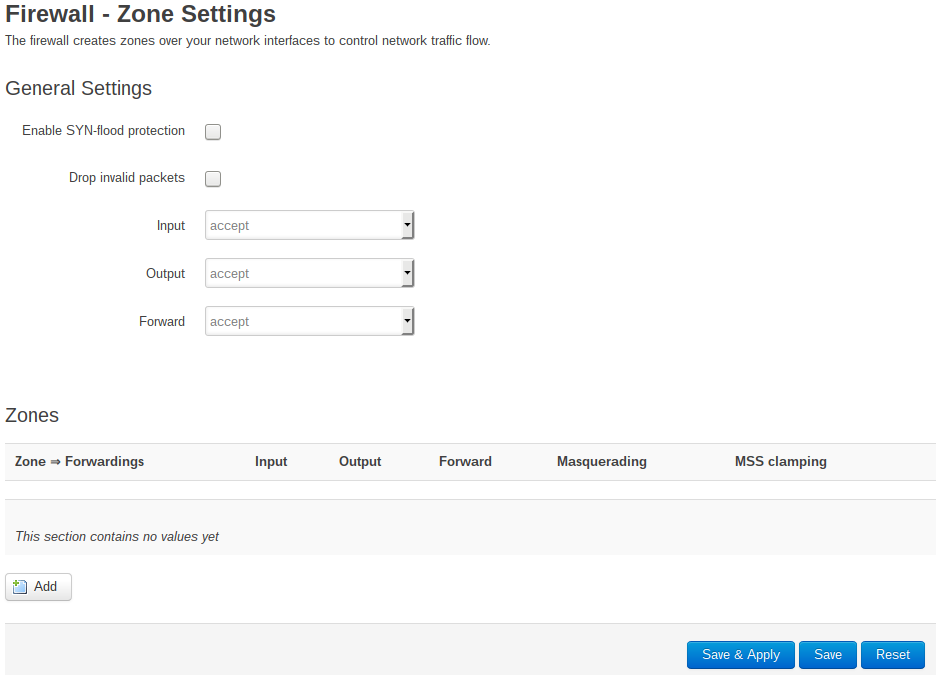
\includegraphics[width=\textwidth]{images/firewall_zone}
    \caption{Legenda da figura}
    \label{fig:id_figura}    
\end{figure}

\subsection{Subfiguras}

É uma técnica para posicionar várias figuras juntas, como subitens de uma figura maior. Elas podem ser posicionadas lado-a-lado ou uma abaixo da outra. Veja exemplo abaixo.

\begin{figure}[!htb]
    \centering
    % Primeira subfigura
    \begin{subfigure}[b]{0.45\textwidth}
        \centering
        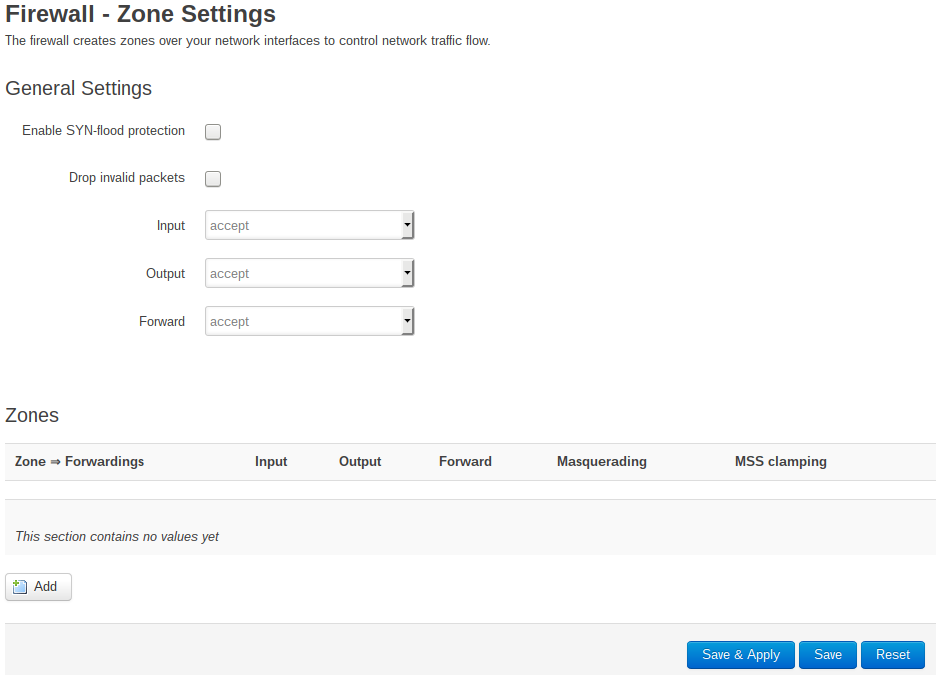
\includegraphics[width=\textwidth]{images/firewall_zone}
        \caption{Legenda da Subfigura 1}
        \label{fig:id_subfig1}
    \end{subfigure}
    \hfill
    % Segunda subfigura
    \begin{subfigure}[b]{0.45\textwidth}
        \centering
        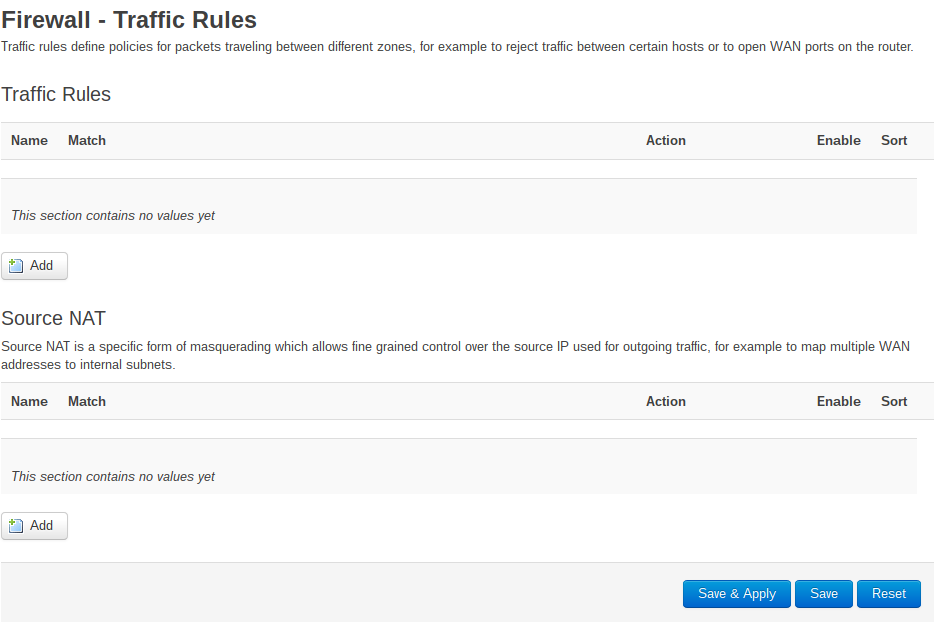
\includegraphics[width=\textwidth]{images/firewall_traffic.png}
        \caption{Legenda da Subfigura 2}
        \label{fig:id_subfig2}
    \end{subfigure}
    \caption{Legenda da Figura Principal (exemplo lado-a-lado)}
    \label{fig:id_figura_principal}
\end{figure}

\section{Tabelas}

\verb@\begin{tabular}{|c|c|c|}@: Cria uma tabela com três colunas centralizadas (c), com bordas verticais entre elas.

\verb@\multicolumn{2}{|c|}{Texto}@: Mescla duas colunas (2) e as alinha centralizadas (c), com bordas verticais ao redor.

\verb|\multirow{2}{*}{Texto}|: Mescla duas linhas (2), ocupando uma única célula na coluna, e alinha o texto ao centro verticalmente (padrão). O * permite que a largura da célula seja ajustada automaticamente.

\verb|\hline|: Insere uma linha horizontal.

\verb|\cline{2-3}|: Desenha uma linha horizontal que cobre apenas as colunas 2 e 3, usada para delinear células não mescladas.

\begin{table}[!htb]
\centering
\begin{tabular}{|c|c|c|}
\hline
Coluna 1 & Coluna 2 & Coluna 3 \\
\hline
Dado 1   & Dado 2   & Dado 3   \\
\hline
Dado 4   & Dado 5   & Dado 6   \\
\hline
Dado 7   & Dado 8   & Dado 9   \\
\hline
\end{tabular}
\caption{Exemplo de Tabela Simples}
\label{tab:tabela_simples}
\end{table}

\subsection{Tabelas com celulas mescladas (horizontal)}

Exemplo de tabela com celulas mescladas na horizontal:

\begin{table}[!htb]
\centering
\begin{tabular}{|c|c|c|}
\hline
Coluna 1 & \multicolumn{2}{|c|}{Colunas 2 e 3 Mescladas} \\
\hline
Dado 1 & Dado 2 & Dado 3 \\
\hline
\multicolumn{2}{|c|}{Células 1 e 2 Mescladas} & Dado 6 \\
\hline
Dado 7  & \multicolumn{2}{|c|}{Células 2 e 3 Mescladas} \\
\hline
\end{tabular}
\caption{Exemplo de Tabela com Células Mescladas Horizontalmente}
\label{tab:tabela_horizontal}
\end{table}

\subsection{Tabelas com celulas mescladas (vertical)}

Exemplo de tabela com celulas mescladas na vertical:

\begin{table}[!htb]
\centering
\begin{tabular}{|c|c|c|}
\hline
\multirow{2}{*}{Célula Mesclada na Vertical} & Coluna 2 & Coluna 3 \\ 
\cline{2-3}
         & Dado 2   & Dado 3   \\
\hline
Dado 4   & Dado 5   & Dado 6   \\
\hline
Dado 7   & Dado 8   & Dado 9   \\
\hline
\end{tabular}
\caption{Exemplo de Tabela com Células Mescladas Verticalmente}
\label{tab:tabela_vertical}
\end{table}

\section{Notas de Rodapé}

Texto com nota de rodapé.\footnote{Este é um exemplo de nota de rodapé.}

\section{Pseudocódigo}

O Algoritmo~\ref{alg:id_algoritmo} do pseudocodigo segue abaixo:

\begin{algorithm}
\caption{Algoritmo de Exemplo com IF e FOR}
\label{alg:id_algoritmo}
\begin{algorithmic}[1] % O [1] indica que as linhas serão numeradas
    \State $a \gets 0$ \Comment{Inicializa a variável $a$ com 0}
    \State $b \gets 1$ \Comment{Inicializa a variável $b$ com 1}
    \State $n \gets 10$ \Comment{Define o número de iterações do loop}
    
    \For{$i \gets 1$ \textbf{to} $n$} \Comment{Inicia um loop de 1 até $n$}
        \If{$a < b$} \Comment{Condição IF: verifica se $a$ é menor que $b$}
            \State $c \gets a + b$ \Comment{Se a condição for verdadeira, calcula $c = a + b$}
        \Else
            \State $c \gets a - b$ \Comment{Se a condição for falsa, calcula $c = a - b$}
        \EndIf
        \State $a \gets b$ \Comment{Atualiza $a$ para o valor de $b$}
        \State $b \gets c$ \Comment{Atualiza $b$ para o valor de $c$}
    \EndFor

    \State \textbf{return} $b$ \Comment{Retorna o valor final de $b$}
\end{algorithmic}
\end{algorithm}

\section{Código Python}

O Script~\ref{lst:id_codigo_python} segue abaixo:

\begin{lstlisting}[language=Python, caption={Exemplo de Código Python}, frame=single, label={lst:id_codigo_python}]
# Este é um exemplo de código Python
def fibonacci(n):
    """Retorna a sequência de Fibonacci até n."""
    a, b = 0, 1
    while a < n:
        print(a, end=' ')
        a, b = b, a + b
    print()

# Chama a função com n = 1000
fibonacci(1000)
\end{lstlisting}

